% use "xelatex -shell-escape report.tex" to compile
\documentclass[titlepage,12pt]{article}
\usepackage{lmodern}
\usepackage{graphicx}
\usepackage{minted}
\setminted{linenos,fontsize=\scriptsize}
\usepackage{amsmath}
\usepackage{amssymb}

\usepackage{algorithm}
\usepackage{algpseudocode}

\usepackage[margin=27mm]{geometry}

\title{\textbf{Dynamic Programming Project} \\ {\small Report for \emph{CSCI-406:
Algorithms} with Dr.~Dinesh Mehta}}
\author{%
    Peter Palumbo \\ {\small\texttt{ppalumbo@mines.edu}} \\[12pt]
    Jack Rosenthal \\ {\small\texttt{jrosenth@mines.edu}} \\[12pt]
    Paul Sattizahn \\ {\small\texttt{psattiza@mines.edu}} \\
}
\date{4 November 2016}

\setlength\parindent{0pt}
\setlength\parskip{6pt plus 2pt minus 2pt}
\let\ge=\geqslant
\let\le=\leqslant

\begin{document}

\maketitle
\section{Introduction}

This report describes our group's dynamic programing solution to a particular
algorithic problem: given a list of events occuring at times $1,\ldots,n$ find
a viewable subset of the events including the last event. The viewer starts at
time 0 and position 0 and has the choice to move at most 1 position for each
time step.

\section{Recursive Formulation}

\begin{itemize}
    \item Let $\mathtt{evset}_p\{t\}$ denote the set containing only $t$ if an event
        at time $t$ occurs at coordinate $p$, otherwise the empty set.
    \item Let $n$ denote the number of events to occur.
    \item Let $c$ denote the coordinate of the last event.
    \item Let $P(t, x)$ be the predicate $n - t \ge |x - c|$.
\end{itemize}

Our recursive formulation for the maximum observable events subset, $m(t, p)$
where $t$ is the current time and $p$ is the current coordinate, is as
follows:

\begin{displaymath}
    m(t, p) = \mathtt{evset}_p\{t\}\, \cup\,
    \begin{cases}
        \emptyset & \text{if}\ t = n \\
        \text{max}_{\text{length}} \left\{m(t + 1, x) :
        x \in \left\{p - 1, p, p + 1\right\} | P(t, x)
        \right\} & \text{otherwise}
    \end{cases}
\end{displaymath}

Using the above recursive formula, the maximum observable events subset for the
problem presented is $m(0, 0)$.

As seen in Figure~\ref{fig:recursive}, this recursive formula can get
expensive. Up to 3 calls of $m$ may be required for each call of $m$ until the
base case is reached. Fortunately, the predicate $P(t, x)$ prevents making
calls for which a solution would be impossible.

\begin{figure}[H]
    \begin{center}
    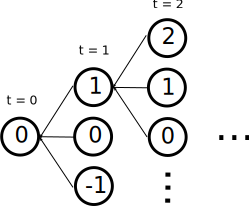
\includegraphics[width=0.4\linewidth]{dp_recursive}
    \end{center}
    \caption{A tree showing the calls of our recursive formula. The
    labels on the nodes show the position of the telescope.}
    \label{fig:recursive}
\end{figure}

\subsection{Recurrence Relation}

It is easy to notice that subtrees in Figure~\ref{fig:recursive} will repeat
frequently in solving the problem. This is illustrated in Figure~\ref{fig:red};
the edges marked in red indicate subtrees which have already been computed and
an intermediate stored result can be used rather that recomputing the subtree.

\begin{figure}[H]
    \begin{center}
    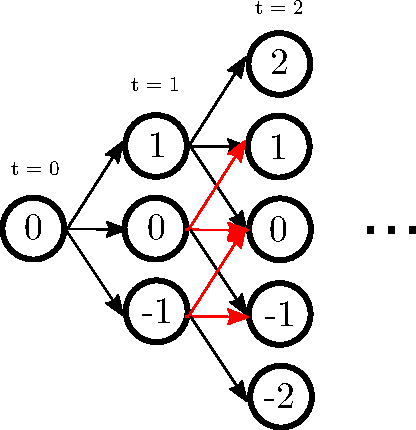
\includegraphics[width=0.4\linewidth]{dp_red}
    \end{center}
    \caption{The same tree as in Figure~\ref{fig:recursive}. Red edges indicate the
    subtrees that the intermediate result can be stored.}
    \label{fig:red}
\end{figure}

\subsection{Pseudocode}

By simply storing completed function calls of $m$ in a dictionary-like
structure, one can implement our dynamic programming method presented. An
example of this is shown below:

\begin{algorithm}
\begin{algorithmic}
    \State{\Comment{$D$ is a global dictionary-like structure}}
    \Function{$m$}{$t$, $p$}
    \If{$(t, p) \in D$}
        \Return{$D[(t, p)]$}
    \ElsIf{$t = n$}
        \Return{$D[(t, p)] = \mathtt{evset}_p\{t\}$}
    \Else
        \State{\Return{%
           $D[(t, p)] = \mathtt{evset}_p\{t\}\, \cup \,
                    \text{max}_{\text{len}} \left\{m(t + 1, x) :
                    x \in \left\{p - 1, p, p + 1\right\} | P(t, x)
                    \right\}$
                }}
    \EndIf
    \EndFunction
\end{algorithmic}
\end{algorithm}

Note that this algorithm creates an \emph{implicit traceback} by using the call
stack alongside stored intermediate results.

\subsection{Algorithmic Complexity}

At each level of the tree in Figure~\ref{fig:red} at a certain time $t$, there
are $2t + 1$ nodes (not taking into account that $P(t, x)$ will reduce this
amount). Once we take into account $P(t, x)$ reducing the amount of calls we
will make, we notice a similar pattern results. Letting $n$ be the number of
events to visit, there is exactly 1 call at $t = n$, 3 calls at $t = n -1$, 5
calls at $t = n - 2$, and so forth. This means that at a certain time $t$, the
number of nodes at that time will also be bounded by $2(n - t) + 1$. Putting
these two bounds together gives the formulation
\begin{displaymath}
    \sum_{i=0}^{\left\lceil \frac{n}{2} \right\rceil} (2i + 1) +
    \sum_{j=0}^{\left\lfloor \frac{n}{2} \right\rfloor} (2j + 1) =
    {\left\lceil\frac{n}{2}\right\rceil}^2 +
    {\left\lfloor\frac{n}{2}\right\rfloor}^2 =
    \left\lceil{\frac{n^2}{2}}\right\rceil \le n^2
\end{displaymath}
as the number of nodes to visit. This leaves us with a worst-case algorithmic
complexity of $O(n^2)$.

\section{Implementation}

Our implementation in the \emph{Python} programming language is as follows:

\inputminted{python3}{dp.py}

\subsection{Examples}

\input examples.tex

\end{document}
